\chapter{Methodology}
The goal of this project is to develop a practical gender bias detection model tailored for real-world MT scenarios. It targets common use cases like translating everyday sentences or job descriptions, focusing on flagging biased language at the sentence level. This means the model evaluates each sentence independently, without considering context from surrounding sentences. This approach guides both the model’s design and the preparation of the training data, where each translation pair is treated as a separate example. The project begins by selecting and combining datasets from previous work (see \autoref{fig:workflow}). The model building phase then follows, as shown in the purple boxes. It starts with cleaning and preparing the data, followed by extracting features for training. A pre-trained \texttt{mBERT} model is then fine-tuned for the classification task. Its performance is measured using standard evaluation metrics. In the final step, the trained model is integrated  into the demo application.

\vspace{1cm} 
\begin{figure}[htb]
    \centering
    \scalebox{0.8}{\tikzstyle{startstop} = [rectangle, rounded corners, minimum width=3cm, minimum height=1cm,text centered, draw=black, fill=gray!20]
\tikzstyle{process} = [rectangle, minimum width=3cm, minimum height=1cm, text centered, draw=black, fill=blue!10]
\tikzstyle{arrow} = [thick,->,>=stealth]

\begin{tikzpicture}[node distance=1.7cm]

\node (start) [startstop] {Select and Combine Datasets};
\node (clean) [process, below of=start] {Clean and Pre-process Data};
\node (features) [process, below of=clean] {Extract Features};
\node (train) [process, below of=features] {Train Model};
\node (evaluate) [process, below of=train] {Evaluate Model Performance};
\node (demo) [startstop, below of=evaluate] {Show Model in Demo Application};

\draw [arrow] (start) -- (clean);
\draw [arrow] (clean) -- (features);
\draw [arrow] (features) -- (train);
\draw [arrow] (train) -- (evaluate);
\draw [arrow] (evaluate) -- (demo);

\end{tikzpicture}
}
    \caption{Methodology Overview}
    \label{fig:workflow}
\end{figure}
\vspace{1cm} 

\section{Dataset}
    Since no ready-to-use dataset existed for this task and no prior work had developed a comparable model, it was necessary to define: (1) the required number of samples, and (2) the desired content of the dataset. For a binary classification task of detecting gender bias using \texttt{mBERT}, general guidelines suggest between 100 and 5,000 labeled samples for fine-tuning \parencite{pecherComparingSpecialisedSmall2024}, while multi-class tasks need fewer samples (around 100). However, the complex nature of gender bias often requires a larger dataset for robust detection since the number of samples depends mainly on the task type. For the final dataset, 2,000 to 5,000 samples were selected to provide enough data for effective training while staying within resource limits.

    Existing EN-DE datasets were reviewed to reduce the need for manual data creation. The following sources were considered: \texttt{\href{https://huggingface.co/datasets/FBK-MT/mGeNTE}{mGeNTE en-de}} \parencite{savoldiMGeNTEMultilingualResource2025}, \texttt{\href{https://github.com/g8a9/building-bridges-gender-fair-german-mt}{Building Bridges Dictionary}} \parencite{lardelliBuildingBridgesDataset2024}, and \texttt{\href{https://research.google/blog/a-dataset-for-studying-gender-bias-in-translation/}{Translated Wikipedia Biographies}} \parencite{stellaDatasetStudyingGender2021}.

    Analysis of the \texttt{Translated Wikipedia Biographies} dataset revealed several issues that prevented direct reuse. In many instances, the \texttt{perceivedGender} column contained subject names instead of expected labels such as \texttt{Male}, \texttt{Female}, or \texttt{Neutral}, making manual verification necessary. Additionally, all examples were labeled as neutral (0), as the dataset was designed around correctly gendered references. Since the remaining two datasets were already balanced and contained a sufficient number of neutrally gendered examples, the Wikipedia Biographies dataset was excluded from the final training data. \texttt{mGeNTE} contains naturally occurring sentences with gendered entities, while \texttt{Building Bridges} focuses on German GFL entries for explicitly gendered nouns such as professions. 

\begin{table}[ht!]
    \centering
    \renewcommand{\arraystretch}{1.3}
    \begin{tabularx}{\textwidth}{|>{\raggedright\arraybackslash}X|>{\raggedright\arraybackslash}X|>{\raggedright\arraybackslash}X|}
    \hline
    \textbf{Dataset} & \textbf{Description} & \textbf{Content} \\ \hline
    \texttt{mGeNTE en-de} \parencite{savoldiMGeNTEMultilingualResource2025} & Multilingual dataset to assess gender bias in MT. & \textasciitilde1,500 gender-ambiguous and gendered English sentences with gender-neutral and gendered German translations. \\ \hline
    \texttt{Building Bridges Dictionary} \parencite{lardelliBuildingBridgesDataset2024} & Bilingual dictionary designed to support gender-fair EN-DE translation. & \textasciitilde230 German gender-neutral and gender-inclusive singular and plural sentences with English equivalents. \\ \hline
    \end{tabularx}
    \caption{Overview of suitable EN-DE datasets based on past works}
    \label{tab:available_datasets}
\end{table}

\subsection{Pre-processing}

\subsubsection{mGeNTE en-de} 
The mGeNTE dataset contained the following relevant information:  

\begin{itemize}  
  \item \texttt{SET-G}: English sentences with a clearly gendered subject.  
  \item \texttt{SET-N}: English sentences with neutral or ambiguous subject gender.  
  \item \texttt{REF-G}: German translations that preserve or introduce gender.  
  \item \texttt{REF-N}: German translations that are fully gender–neutral.  
\end{itemize}  

\noindent
The bias definition used in this study classifies translations that omit the original gender as neutral, as they do not rely on a male default or stereotype. Although gender-neutral translations may be imperfect, they are not considered biased within this framework. Initial experiments indicated that including \texttt{REF-N} pairs during training led to over-penalization of neutral outputs. Due to the limited availability of neutral examples, such outputs were not penalized in the final training setup. Each original entry was split into two paired examples and labeled as follows:  
\[
\begin{aligned}
\texttt{SET\!-\!G} + \texttt{REF\!-\!G} &\;\rightarrow\; 0 \quad(\text{neutral})\\
\texttt{SET\!-\!G} + \texttt{REF\!-\!N} &\;\rightarrow\; 0 \quad(\text{neutral})\\
\texttt{SET\!-\!N} + \texttt{REF\!-\!N} &\;\rightarrow\; 0 \quad(\text{neutral})\\
\texttt{SET\!-\!N} + \texttt{REF\!-\!G} &\;\rightarrow\; 1 \quad(\text{biased})
\end{aligned}
\]  
This procedure yields 3,000 total instances, of which 750 are labeled biased (1) and 2,250 are labeled neutral (0).\footnote{The transformed dataset can be found in \texttt{/datasets/mgente\_final.csv}.} 

\subsubsection{Building Bridges Dictionary} 
This dataset consisted of a GFL dictionary of nouns, not full sentences. That made it useful for studying GFL, but not suitable for this task, which requires sentence-level context. To address this, prompt engineering was used with Google Gemini 2.5 Flash to synthetically expand the dataset\footnote{Refer to Appendix~\ref{appendix:gemini_prompt} for the prompt.}. Nouns from the original dataset were used to create multiple grammatically correct sentence variations, covering singular, plural, gender-neutral, and gender-inclusive forms. The dataset uses the star form (e.g., \textit{Lehrer*innen}) as its inclusive format. Since the colon form (e.g., \textit{Lehrer:innen}) is also common in practice, a script was used to duplicate all entries with stars and replace the star with a colon to generate additional variants. This resulted in 3,381 total entries: 2,001 labeled as 0 (neutral) and 1,380 labeled as 1 (biased).\footnote{The transformed dataset can be found in \texttt{/datasets/lardelli\_final.csv}.}

\subsubsection{Tatoeba} 

The aforementioned setup lacked genuinely neutral examples, defined as sentences without any gendered subject, such as "The weather is nice" or "How are you". Including such cases is important for training the model to recognise that not all translations are relevant for gender bias detection, and that many sentences should be classified as neutral. As no suitable dataset for this category was available, a supplementary set was created from random EN–DE sentence pairs drawn from the \texttt{\href{https://tatoeba.org/en/}{Tatoeba}} corpus. A total of 550 sentence pairs was sampled. Manual filtering was applied to these samples to remove any pairs containing incorrect translations or stereotypical gendering, as public contributions often default to male forms. The final subset contained 532 clearly neutral sentence pairs, all labelled with 0.\footnote{The transformed dataset can be found in \texttt{/datasets/tatoeba\_final.csv}.}


\subsubsection{Available Data Summary}

\autoref{tab:data-summary} shows an overview of the labeled data from the three available sources. 

\begin{table}[H]
\centering
\begin{tabularx}{\textwidth}{l *{3}{>{\centering\arraybackslash}X}}
\toprule
\textbf{Dataset} & \textbf{Total} & \textbf{Neutral (0)} & \textbf{Biased (1)} \\
\midrule
\texttt{lardelli\_final.csv} & 3381 & 2001 & 1380 \\
\texttt{mgente\_final.csv}   & 3000 & 2250 & 750  \\
\texttt{tatoeba\_final.csv}      & 532  & 532  & 0    \\
\bottomrule
\end{tabularx}
\caption{Summary of available labeled examples}
\label{tab:data-summary}
\end{table}

The number of samples selected from each dataset was determined through iterative testing. Multiple dataset variants were created by upsampling or downsampling specific groups. The documentation of this process is discussed in \autoref{subsection:hyperparameter_tuning_methodology}.

\subsection{Data Splitting and Cleaning}
    The dataset is partitioned into training (80\%), validation (10\%), and test (10\%) subsets. This splitting ratio follows established practices commonly employed in ML experiments \parencite{bahetiTrainTestValidation2021}. It provides enough samples for the model to learn general patterns while reserving separate subsets for tuning and final evaluation. Stratified sampling was used to maintain consistent label distribution (biased vs. neutral) across all three sets. For example, if 30\% of the full dataset is biased, each split will also have 30\% biased samples. 

    Advanced text cleaning steps (punctuation removal, lowercasing, or stemming) were not applied due to the use of \href{https://huggingface.co/google-bert/bert-base-multilingual-cased}{\texttt{bert-base-multilingual-cased}}. This tokenizer handles raw, unaltered text and retains case distinctions. The model was pretrained on large corpora containing natural language in its original form \parencite{devlinBERTPretrainingDeep2019}, so modifying the input by lowercasing or stripping punctuation could remove meaningful patterns the model has learned to recognize. Steps to handle missing values or invalid entries were already performed in the individual datasets, so they did not need to be repeated when creating the final merged dataset.

\section{Training Pipeline}
    \texttt{mBERT} with a binary classification head is used to predict whether a translation is \textit{biased} or \textit{neutral}. The tokenizer encodes input sentence pairs into numerical representations and distinguishes between source and target sentences. All sequences are padded or truncated to a fixed length of 256 tokens, which preserves most content while keeping processing efficient. The model represents each input pair with a summary vector of the entire sequence, which is then used for classification into the two categories. Each dataset is instantiated and encoded into a format suitable for model input, including the EN–DE sentence pairs and their corresponding labels. Training hyperparameters are established through tuning. The model iteratively learns from the training data by adjusting its parameters to minimize classification errors, with validation performance guiding the process and helping prevent overfitting. At the end of training, the best-performing model is selected based on validation metrics and used for subsequent gender bias detection.

\section{Evaluation Strategy}
    Model evaluation was performed during training using the validation set and after training using two distinct test sets. As detailed in \autoref{subsection:hyperparameters_explained}, the macro F1 score was employed as the primary metric to assess model performance. The validation set served to monitor training progress across epochs, and the checkpoint with the highest validation F1 score was saved. The combined training dataset was handcrafted and had known limitations, so relying solely on the validation set was insufficient to assess final model performance. To better evaluate generalization, a separate handcrafted test set was created. This set contains EN-DE sentence pairs with manually assigned bias labels. Using these two evaluation strategies, both the fine-tuning process and the composition of the combined training dataset were iteratively adjusted to improve model robustness and generalization.

\subsection{Handcrafted Test Set Construction} \label{subsection:eval_dataset}
    The handcrafted test set was developed from a user-centered perspective, focusing on identifying inputs that expose various failure and edge cases. Examples were organized into categories: neutral sentences, neutral sentences containing gendered roles, biased translations, and translations featuring German GFL. It comprises simple synthetic sentences written specifically for this purpose, as well as authentic examples extracted from job postings. The inclusion of real-world data aims to simulate practical use cases, such as evaluating translated job advertisements for gender bias.

    Emphasis was placed on diversity in sentence structure and content rather than maintaining label balance. Certain examples tested the model’s tendency to incorrectly flag neutral sentences containing gendered terms, while others assessed its capacity to detect various GFL forms in German, including terms like “Lehrende” and the colon notation “Lehrer:innen.” Bias labels were assigned manually according to the criteria established in Chapter 2. The complete handcrafted test set, containing 26 labeled translation pairs, is provided in the Appendix.

\subsection{Hyperparameter Selection and Tuning} \label{subsection:hyperparameter_tuning_methodology}
     While a few standard hyperparameters were tested, the focus was placed on tuning dataset composition and the number of frozen layers. These factors showed a significantly stronger influence on model performance during experimentation. Since the training data originated from a mix of external sources with varying quality, adjusting the use and structure of the data was considered more effective than extensive hyperparameter optimization. Recommended default values from prior work provided sufficiently strong baselines and were therefore used as the starting point.

    \paragraph{Epochs} The model was trained for a maximum of 8 epochs, with early stopping enabled using a patience of two epochs. This setup halted training if the macro F1 score did not improve over two consecutive epochs. The approach follows the recommendation by \textcite{pecherComparingSpecialisedSmall2024}, who suggest training until convergence, with a cap of 10 epochs and early stopping. In this case, validation loss typically increased after 8 epochs, with no further improvements observed. Limiting the training to 8 epochs helped mitigate overfitting and reduced training time.

    \paragraph{Batch size} A batch size of 16 was used. This value is commonly applied in fine-tuning scenarios involving small datasets, offering a reasonable balance between memory efficiency and training stability. Smaller batch sizes paired with lower learning rates were tested but led to reduced performance and less effective learning in early epochs. Existing literature, including \textcite{mosbachStabilityFinetuningBERT2021}, supports the use of a batch size of 16; no further experiments with smaller values were conducted.

    \paragraph{Learning rate} The learning rate was set to 2e-5. This value, originally proposed in \textcite{devlinBERTPretrainingDeep2019}, remains widely used for fine-tuning transformer models. Alternatives such as 1e-5 and 3e-5 were evaluated but yielded slightly lower validation scores. The 2e-5 setting showed the most stable and consistent results and was therefore applied in all final training runs.

    \paragraph{Optimizer and scheduler} The \texttt{Trainer} API employed the AdamW optimizer by default. A warmup-linear learning rate schedule was used: the rate gradually increased during the first 10\% of training steps (warmup) and then decreased linearly until completion. This schedule supports smooth learning and helps prevent instability during early training.

\subsection{Training Dataset Tuning} \label{subsection:training_dataset_tuning}
    Since the F1 scores were similar across dataset versions, the main evaluation was based on the handcrafted test set of 26 sentences.\footnote{The detailed documentation of each iteration is included in Appendix \ref{appendix:dataset_tuning_table}. The focus in this section is on the process and rationale rather than on numeric results.} This small test set does not provide a complete indication of overall model quality, but it offers insight into practical usability. Any statements regarding better or worse performance should be considered in light of this limitation.

    The dataset \texttt{mgente\_final} was considered the best source because its samples are natural sentences. All 750 biased samples from \texttt{mgente\_final} were included, along with exactly 750 neutral samples. The tuning process aimed to adjust the remaining datasets to maintain a maximum ratio of 60\% neutral to 40\% biased samples. Sampling was performed using the \texttt{join\_datasets.py} script, which loads the labeled datasets, samples a fixed number of biased and neutral entries per dataset using a fixed random seed (10), and combines them into a single training set. The script also checks for missing values and label integrity before saving the final CSV file. The tuning process across dataset versions, including their composition and rationale, is summarized in \autoref{tab:dataset_versions}.

    The Baseline dataset already achieved strong performance, with a test F1 score of 0.975 and 84.6\% accuracy on the handcrafted test set. However, it failed on some neutral examples such as \textit{"My mother is an engineer." / "Meine Mutter ist Ingenieurin."} (predicted biased with confidence 0.55) and on certain German GFL patterns (e.g., double naming and the colon notation). Adjustments made to the dataset composition in Datasets B through E occasionally improved specific weaknesses. In one case, Dataset E succeeded in correctly classifying a neutral gendered sentence that the Baseline had misclassified. At the same time, these targeted improvements often introduced new issues, such as misclassifications in job advertisement examples. The changes did not produce consistent gains on the handcrafted test set and in some cases reduced overall accuracy. As a result, the Baseline dataset composition was used for final training, as it offered the most reliable balance between targeted performance and general usability.

\vspace{0.8em}
\begin{table}[ht]
    \centering
        \begin{tabularx}{\textwidth}{l X >{\raggedright\arraybackslash}X}
    \toprule
    \textbf{Dataset} & \textbf{Rationale} & \textbf{Sample Distribution (biased/neutral)} \\
    \midrule
    A & Initial setup using equal parts of \texttt{mgente\_final} and \texttt{lardelli\_final}, with some \texttt{tatoeba\_final} neutrals. & mgente 750 / 750, lardelli 750 / 750, tatoeba 0 / 250 \\
    B & Built on A. Increased \texttt{lardelli\_final} neutrals to better capture GFL patterns and added more \texttt{tatoeba\_final} neutrals. & mgente 750 / 750, lardelli 750 / 1000, tatoeba 0 / 400 \\
    C & Built on A and B. Reduced \texttt{lardelli\_final} biased examples to counter possible overrepresentation. & mgente 750 / 750, lardelli 400 / 750, tatoeba 0 / 250 \\
    D & Built on A and C. Further improved neutral recognition by adding more \texttt{tatoeba\_final} neutral sentences. & mgente 750 / 750, lardelli 750 / 750, tatoeba 0 / 500 \\
    E & Built on A and C. Increased \texttt{mgente\_final} neutral data to raise diversity from naturalistic examples. & mgente 750 / 1,250, lardelli 750 / 750, tatoeba 0 / 250 \\
    \bottomrule
    \end{tabularx}
    \caption[Dataset iterations with rationale and composition]{Dataset iterations with rationale and composition. Each version builds on the Baseline and previous adjustments. Format: source biased / neutral}
    \label{tab:dataset_versions}
\end{table}


\subsection{Layer Freezing Tuning}
    All dataset tuning experiments described above were conducted with layer freezing set to $n=8$, meaning that encoder layers 0 through 7 of \texttt{mBERT} were frozen during training. As explained in \autoref{subsection:hyperparameters_explained}, earlier studies have shown that the middle layers are most semantically informative, while lower layers tend to capture syntactic information. Freezing up to layer 8 was chosen as a baseline to reduce training time while still allowing the model to adapt higher-level representations to the task.Since the results with $n=8$ were already promising, only two further variations were tested: $n=7$ and $n=6$. These settings freeze fewer layers, meaning more of the network remains trainable. The purpose of these tests was to evaluate whether this added flexibility improved performance without overfitting.

    \vspace{0.8em}
    \begin{table}[ht]
        \centering
        \begin{tabularx}{\linewidth}{Xcc}
        \toprule
        \textbf{Frozen Layers} & \textbf{Test F1 (weighted)} & \textbf{Handcrafted Test Set Accuracy} \\
        \midrule
        $n=6$ (layers 0--5 frozen) & 0.981 & 0.808 \\
        $n=7$ (layers 0--6 frozen) & 0.979 & 0.808 \\
        $n=8$ (layers 0--7 frozen) & 0.966 & 0.846 \\
        \bottomrule
        \end{tabularx}
        \caption{Comparison of layer freezing settings}
    \end{table}

    Freezing fewer layers led to slightly higher F1 scores on the test set, but the model with $n=8$ frozen layers achieved the best results on the handcrafted test sentences, which were designed to reflect real-world usability. Since the F1 differences were minor and freezing more layers results in a simpler and more efficient model, $n=8$ was chosen as the final setting.

\section{Demo Application Design}
    The demo application comprises three modules: the user interface, the bias detection model, and the translation component (see \autoref{fig:component_diagram}). Both input modes converge on a common prediction pipeline. On launch, the application loads the trained model and its encoding mechanism into memory. Users can either input raw English text (Tab 1), which is split into sentences and translated into German, or provide aligned EN-DE sentence pairs (Tab 2). Both approaches result in a set of sentence pairs ready for bias analysis. The bias detection pipeline processes these sentence pairs by converting each pair into a representation suitable for the model, which in turn predicts whether a translation is biased or neutral. Predictions are accompanied by a confidence score, which is the probability assigned by mBERT to the predicted label. Results are displayed alongside the original and translated sentences. If bias is detected above a defined threshold, a warning is shown; otherwise, the sentence pair is marked as neutral. Each result is separated to maintain readability.

    \vspace{0.8em}
    \begin{figure}[htb]
    \centering
    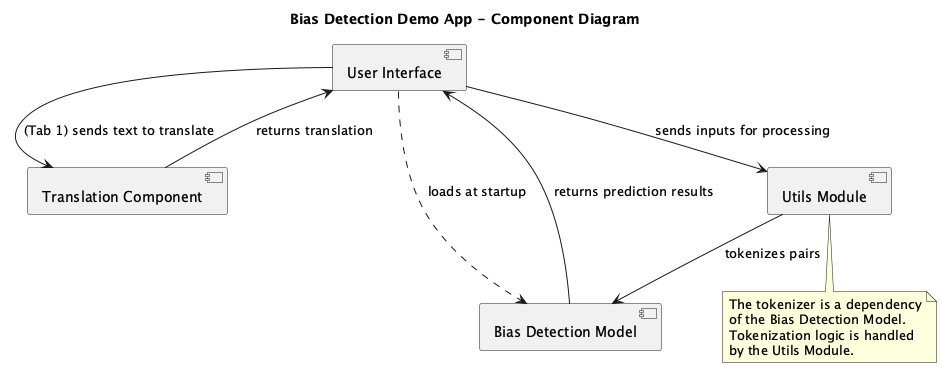
\includegraphics[width=1\textwidth]{modules.png}
    \caption[Component Diagram]{Component Diagram. High-level architecture of the bias detection demo app showing components, their relationships, and data flow}
    \label{fig:component_diagram}
    \end{figure}

    The interface has two main modes (see Figures~\ref{fig:sequence_diagram_1}, \ref{fig:sequence_diagram_2}). In automatic translation, raw English text is submitted, segmented into sentences, and translated. Each sentence is paired with its translation before analysis. In manual pairing, users provide EN-DE sentence pairs directly, which bypasses translation and proceeds to bias evaluation. The system is designed to demonstrate the end-to-end process of bias detection independently of implementation details. The methodology allows the translation component or model representation to be replaced with alternative approaches. The focus is on showing how input sentences are converted into pairs, analyzed for bias, and presented in a user-friendly way. 

    \vspace{0.8em}
    \begin{figure}[H]
    \centering
    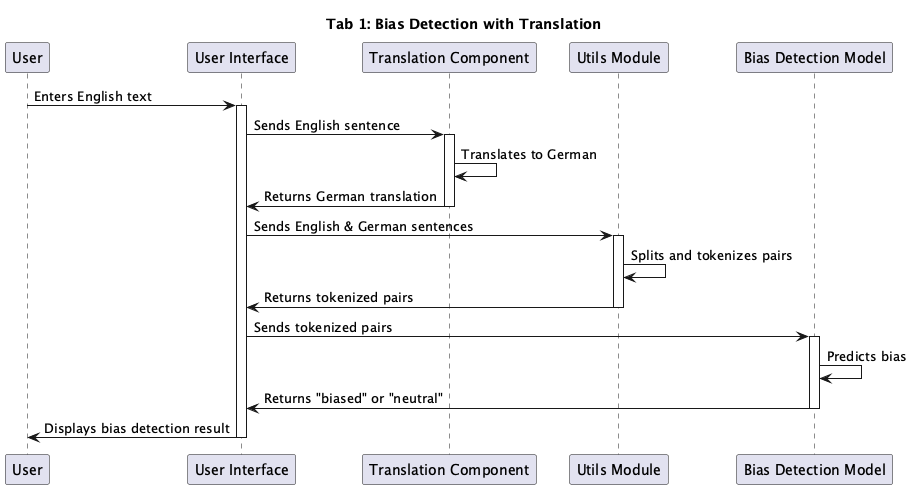
\includegraphics[width=0.95\textwidth]{modules_001.png}
    \caption[Sequence Diagram – Tab 1 (with translation)]{Sequence Diagram – Tab 1 (with translation). Step-by-step flow for Tab 1, showing how user input is translated, tokenized, and processed by the bias detection model}
    \label{fig:sequence_diagram_1}
    \end{figure}

    \begin{figure}[H]
    \centering
    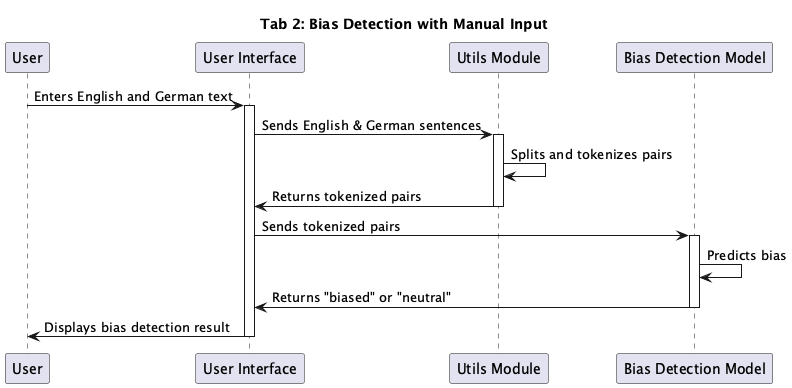
\includegraphics[width=0.95\textwidth]{modules_002.png}
    \caption[Sequence Diagram – Tab 2 (manual input)]{Sequence Diagram – Tab 2 (manual input). Step-by-step flow for Tab 2, showing how manually entered English and German sentences are tokenized and processed by the bias detection model}
    \label{fig:sequence_diagram_2}
    \end{figure}
